\documentclass[Thesis.tex]{subfiles}
\begin{document}

\section*{Variational Methods for Discrete Surface Parameterization. Applications and Implementation.}
Stefan Sechelmann
\subsection*{Zusammenfassung in deutscher Sprache}

Diskret konforme \"{A}quivalenz von Dreiecksnetzen wurde von Luo eingef{\"u}hrt~\cite{Luo2004:Yamabe} und von Springborn {\it et al.}~\cite{Springborn2008} sowie Bobenko {\it et al.}~\cite{BPS2015:dconf} ausf{\"u}hrlich behandelt.
Zwei euklidische Triangulierungen mit gleicher Konnektivit\"{a}t sind diskret konform \"{a}quivalent, wenn es  Faktoren pro Ecke gibt, so dass entsprechende Kanten bis auf Multiplikation mit den Faktoren die gleiche L\"{a}nge haben.
Die konforme Abbildung von triangulierten Fl\"{a}chen auf ebene Gebiete ist mit Hilfe eines Variationsprinzips auf den Skalierungsfaktoren formuliert.

%\begin{figure}[H]
%\centering
%\resizebox{\textwidth}{!}{
%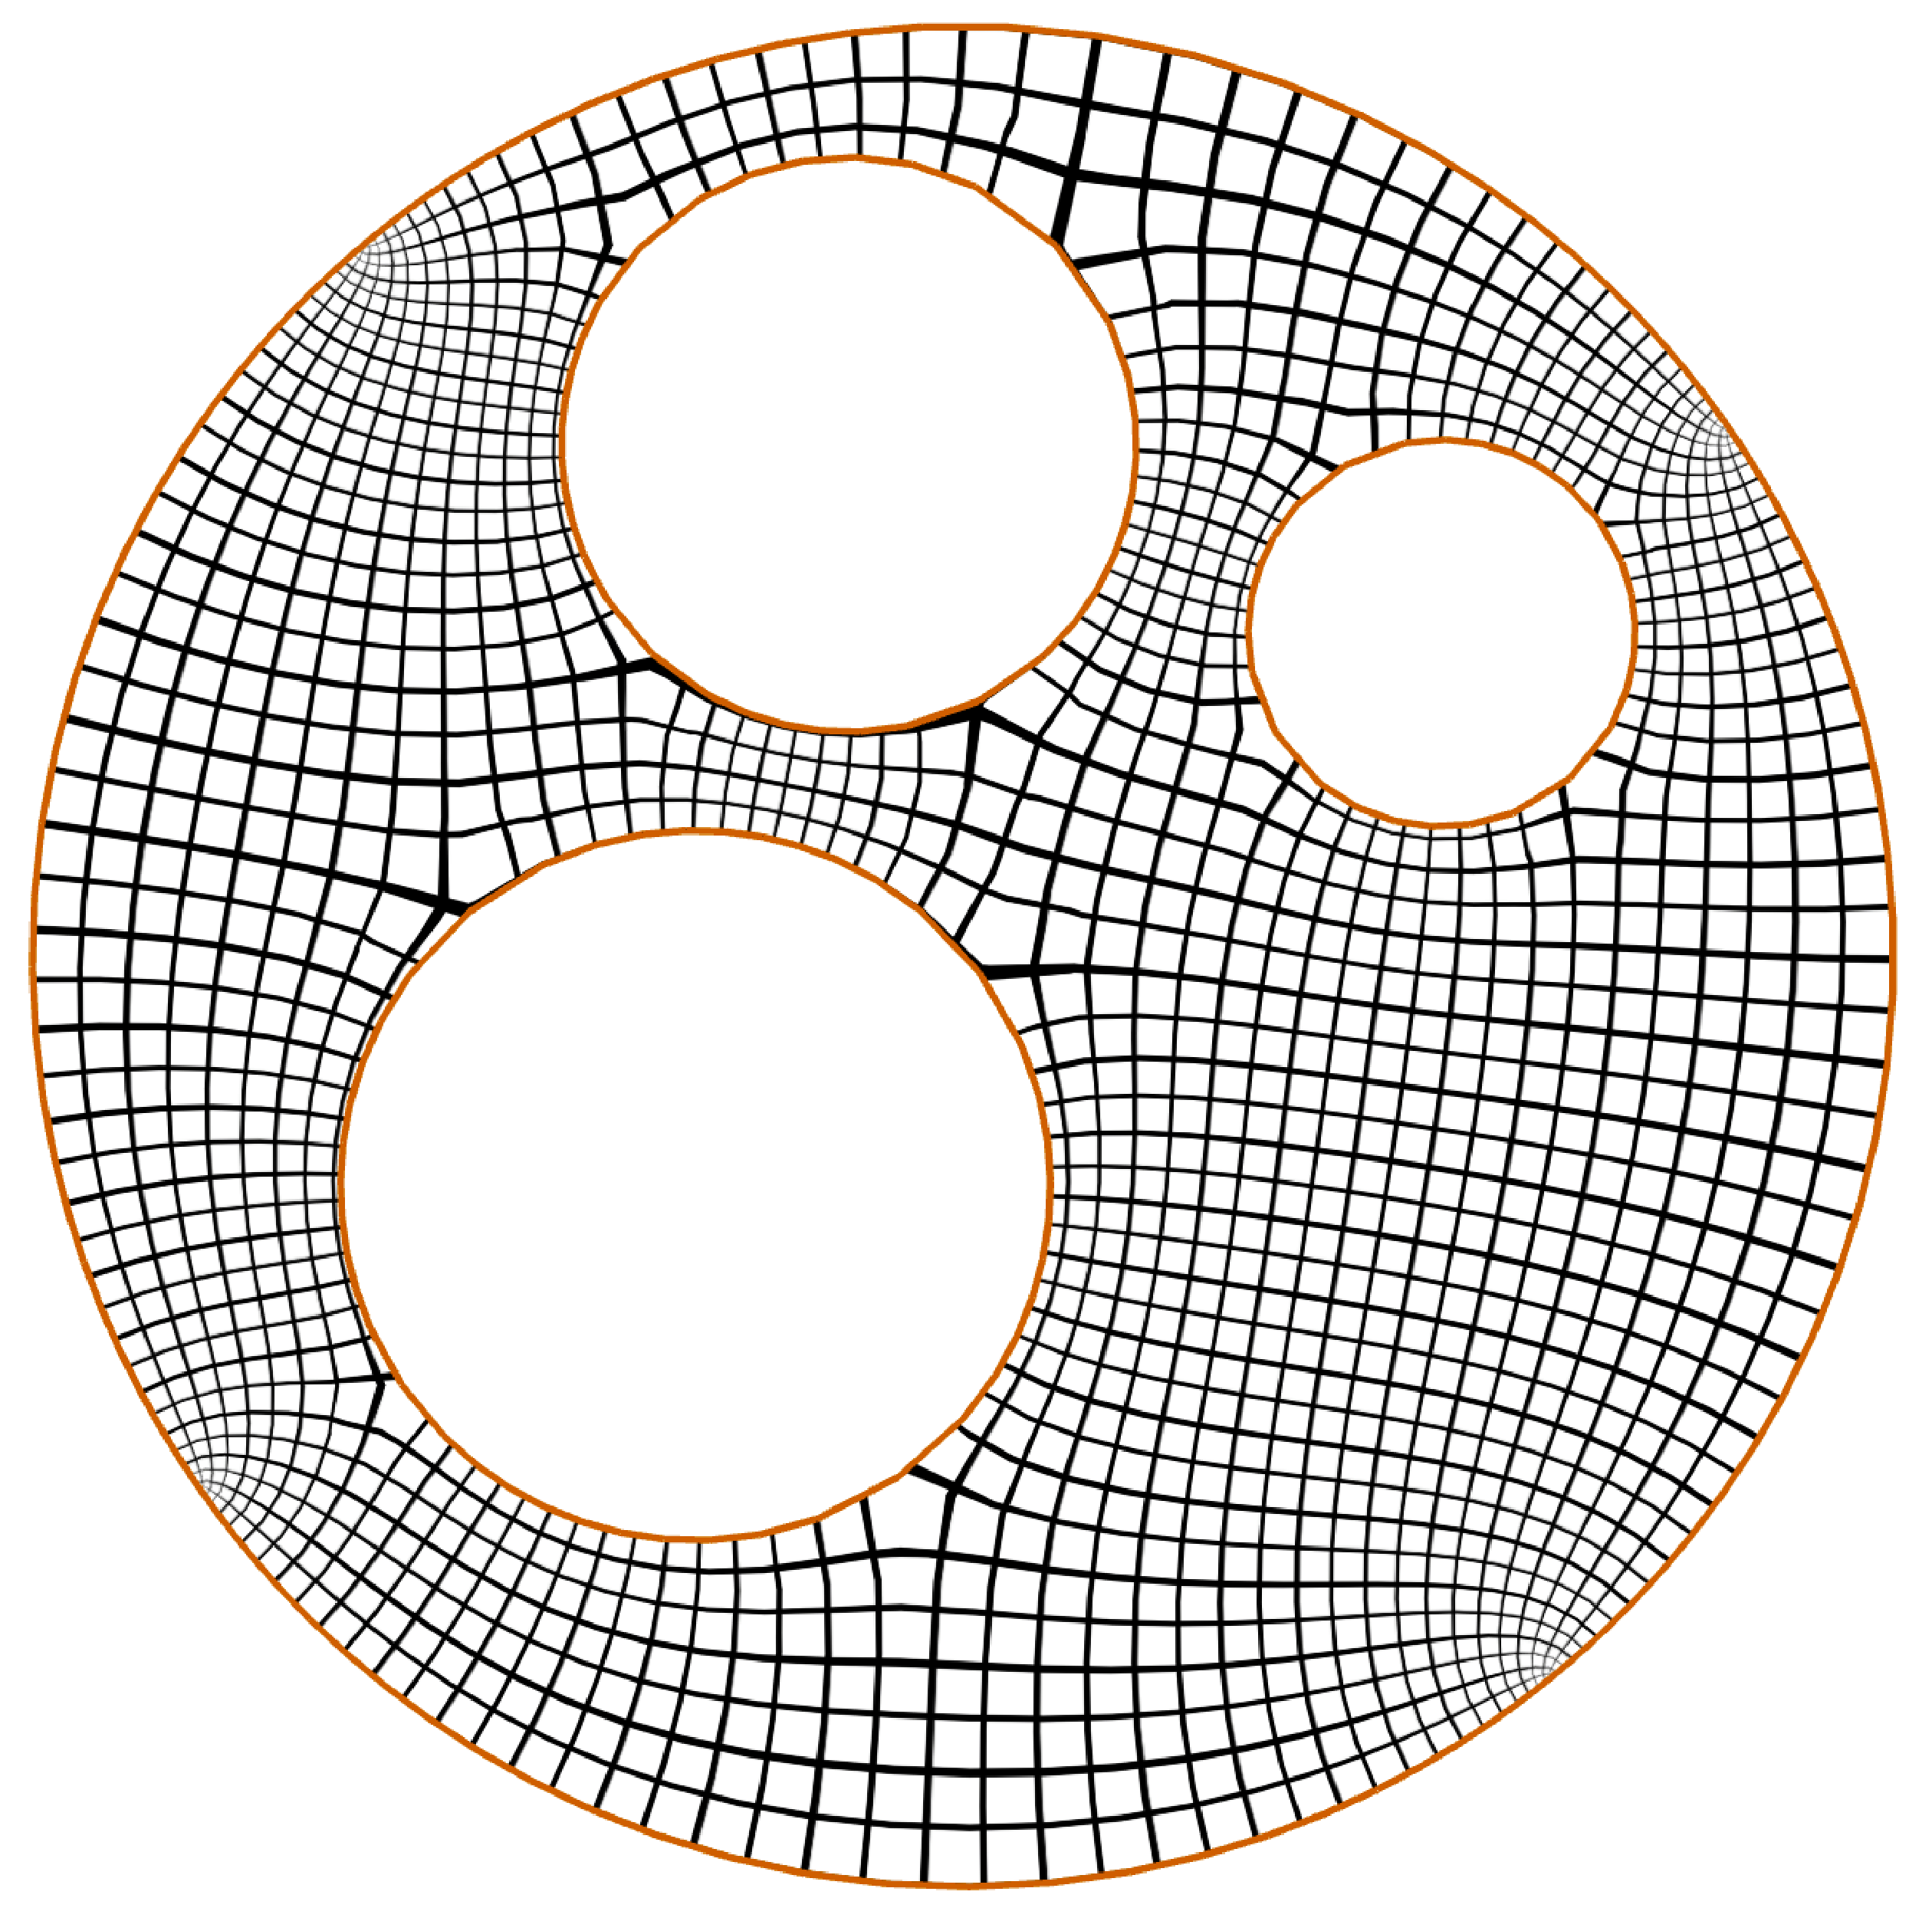
\includegraphics[height=4.8cm]{circle_domain_euclidean/three_holes_map.pdf}
%\raisebox{0.25cm}{
%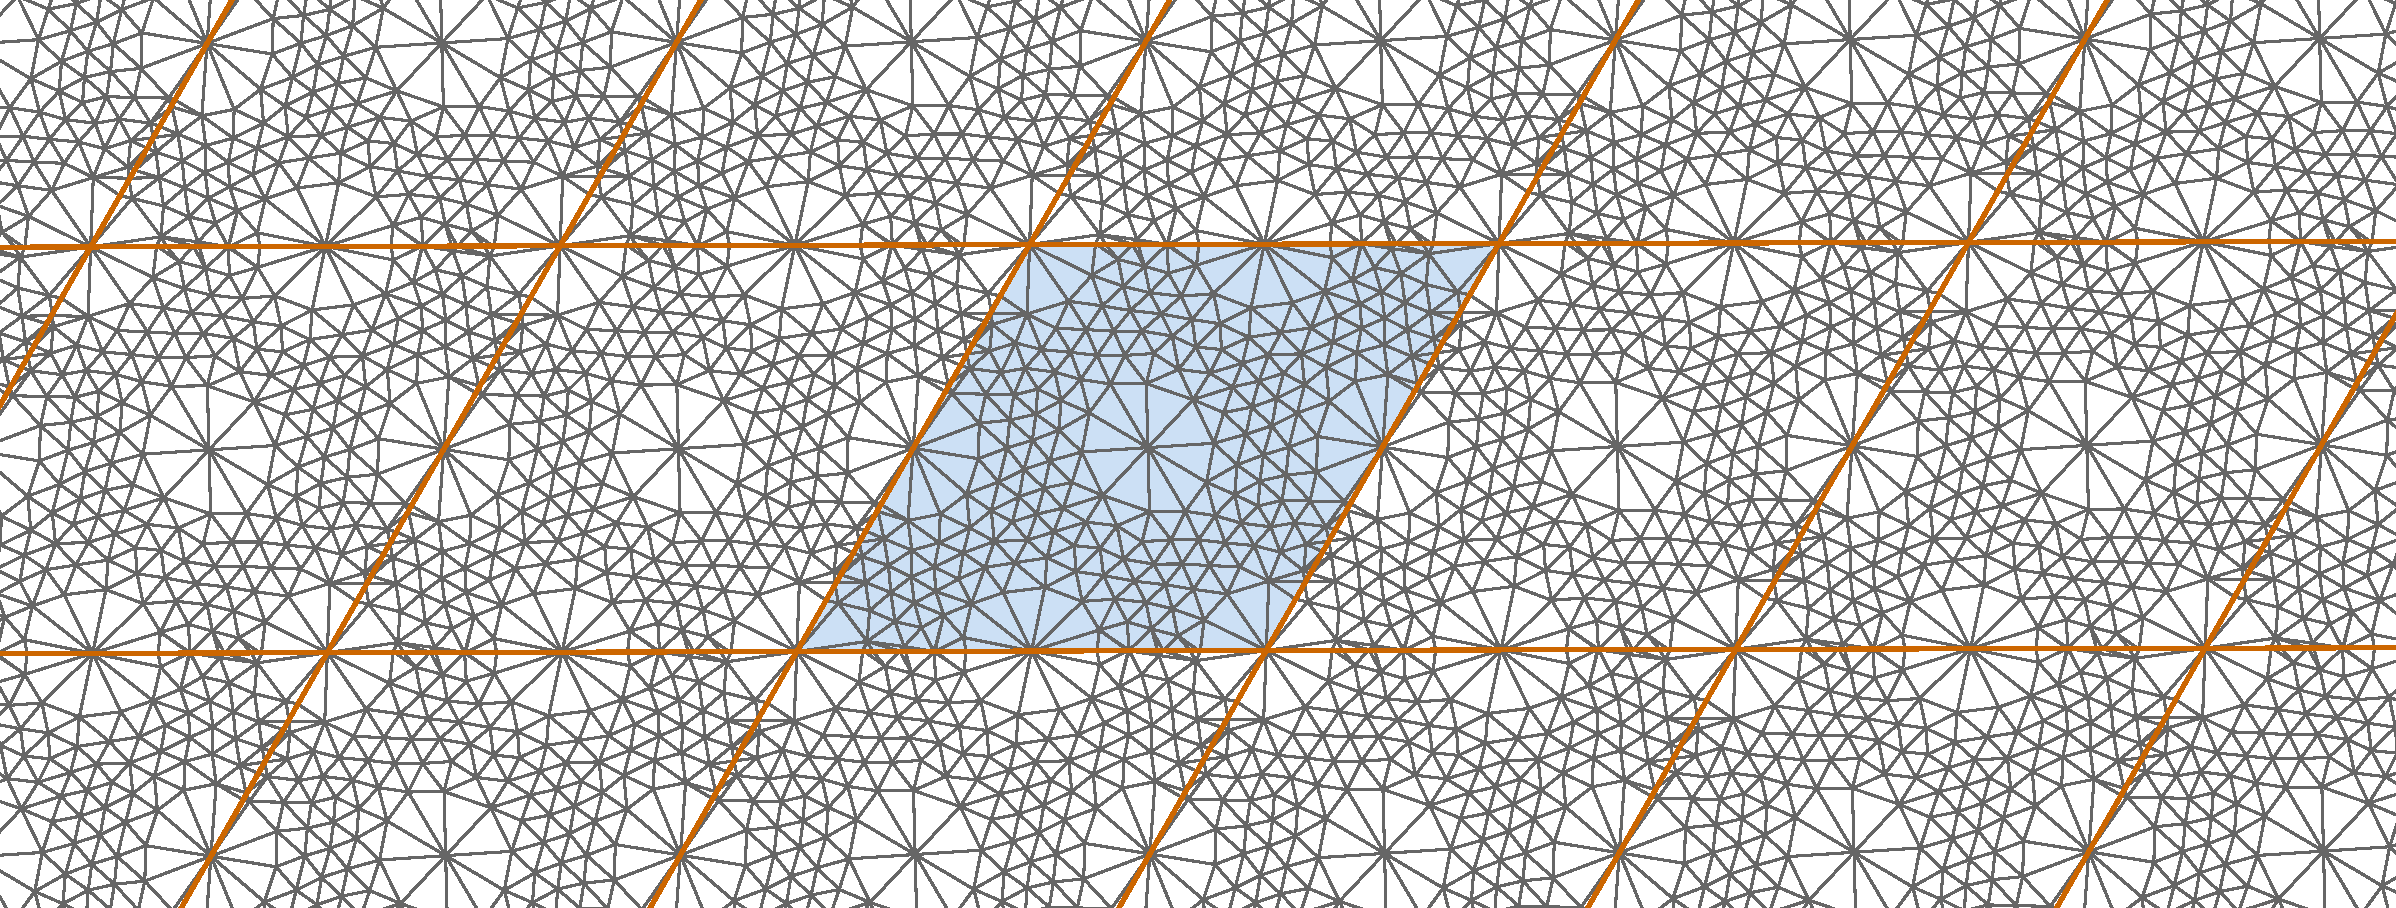
\includegraphics[height=4.5cm]{elliptic_curves/tetrahedron.pdf}
%}
%\includegraphics[height=5cm]{data/hyperelliptic_g3/cover_mesh}
%}
%\caption{
%\it Diskrete Uniformisierungen von Riemannschen Fl\"{a}chen. 
%Links: Ein Gebiet mit vier Randkomponenten wird auf einen von Kreisen begrenzten Bereich abgebildet, siehe Abschnitt~1.5.1.
%Mitte: Uniformisierung einer diskret elliptischen Kurve. Das Bild ist ein flacher Torus, siehe Abschnitt~1.7.2.
%Rechts: Uniformisierung einer hyperelliptischen algebraischen Kurve mit einem regul\"{a}ren Fundamentalpolygon, siehe Abschnitt~1.8.3.
%}
%\label{fig:intro_uniformizations} 
%\end{figure}

Wir konzentrieren uns in dieser Abhandlung auf die experimentellen Aspekte der Theorie und st\"{u}tzen uns dabei auf die theoretischen Grundlagen aus den genannten Arbeiten.
Ganz im Geiste der diskreten Differentialgeometrie untersuchen wir Aussagen und Konstruktionen aus der Differentialgeometrie von glatten Fl\"{a}chen und versuchen diese in den diskreten Strukturen wieder zu finden.

Diese Abhandlung ist in drei Teile aufgeteilt, wovon der erste die konformen Abbildungen behandelt, der andere Anwendungen der Selbigen in der Architektur enth\"{a}lt und der dritte die Implementation der verwendeten Methoden in einer Software beschreibt.

Im ersten Teil beschreiben wir die diskrete Uniformisierung von Riemannschen Fl\"{a}chen mittels diskret konformer \"{A}quivalenz von zyklisch polyedrischen Fl\"{a}chen.
Wir verallgemeinern daf\"{u}r die bekannte Theorie der diskret konformen Dreiecksnetze auf zyklisch polyedrische Fl\"{a}chen.
%Dieser Teil der Theorie wurde in vorangegangenen Arbeiten nur kurz ber\"{u}hrt.
%Weiter beleuchten wir den sph\"{a}rischen Teil der Theorie, welcher bisher nicht behandelt worden ist.
Dieser Teil enth\"{a}lt einen Satz \"{u}ber hyperelliptische Riemannsche Fl\"{a}chen: 
Eine Riemannsche Fl\"{a}che ist hyperelliptisch genau dann, wenn es eine Basis der Uniformisierungsgruppe gibt, deren hyperbolische Achsen sich in einem gemeinsamen Punkt schneiden.
% siehe auch Abbildung~\ref{fig:intro_uniformizations} rechts.
%Die Methoden aus diesem Abschnitt bilden die Grundlage f\"{u}r die Anwendungen in Teil~II.

%\begin{figure}
%\centering
%\resizebox{\textwidth}{!}{
%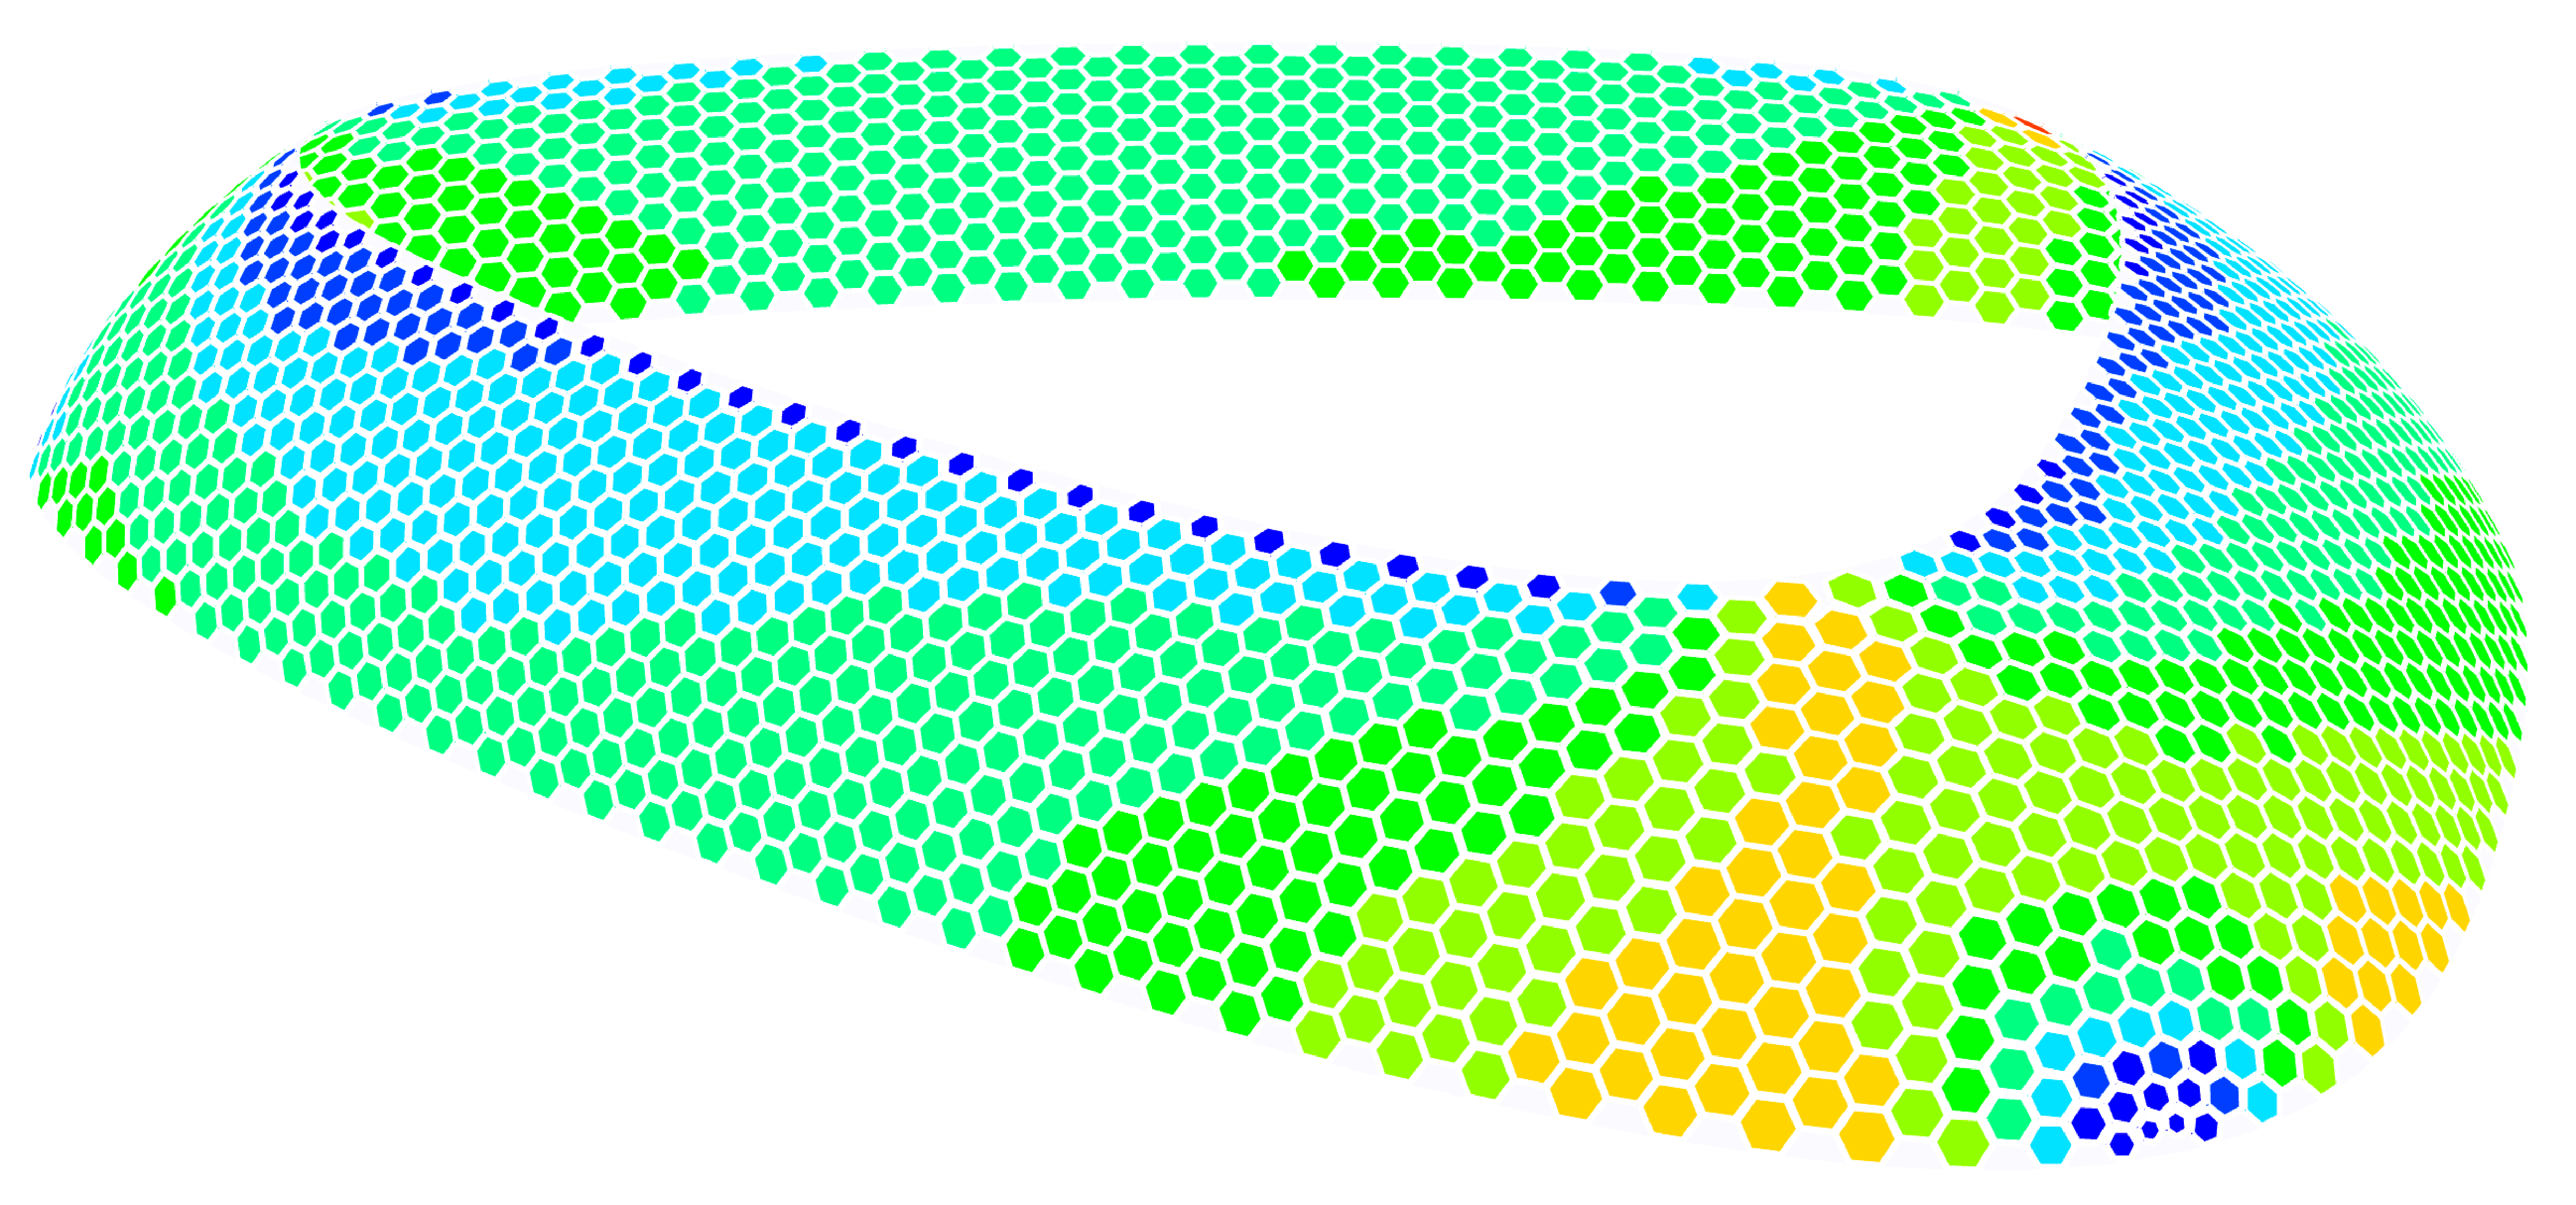
\includegraphics[height=4cm]{images/quantized_singularities5.pdf}
%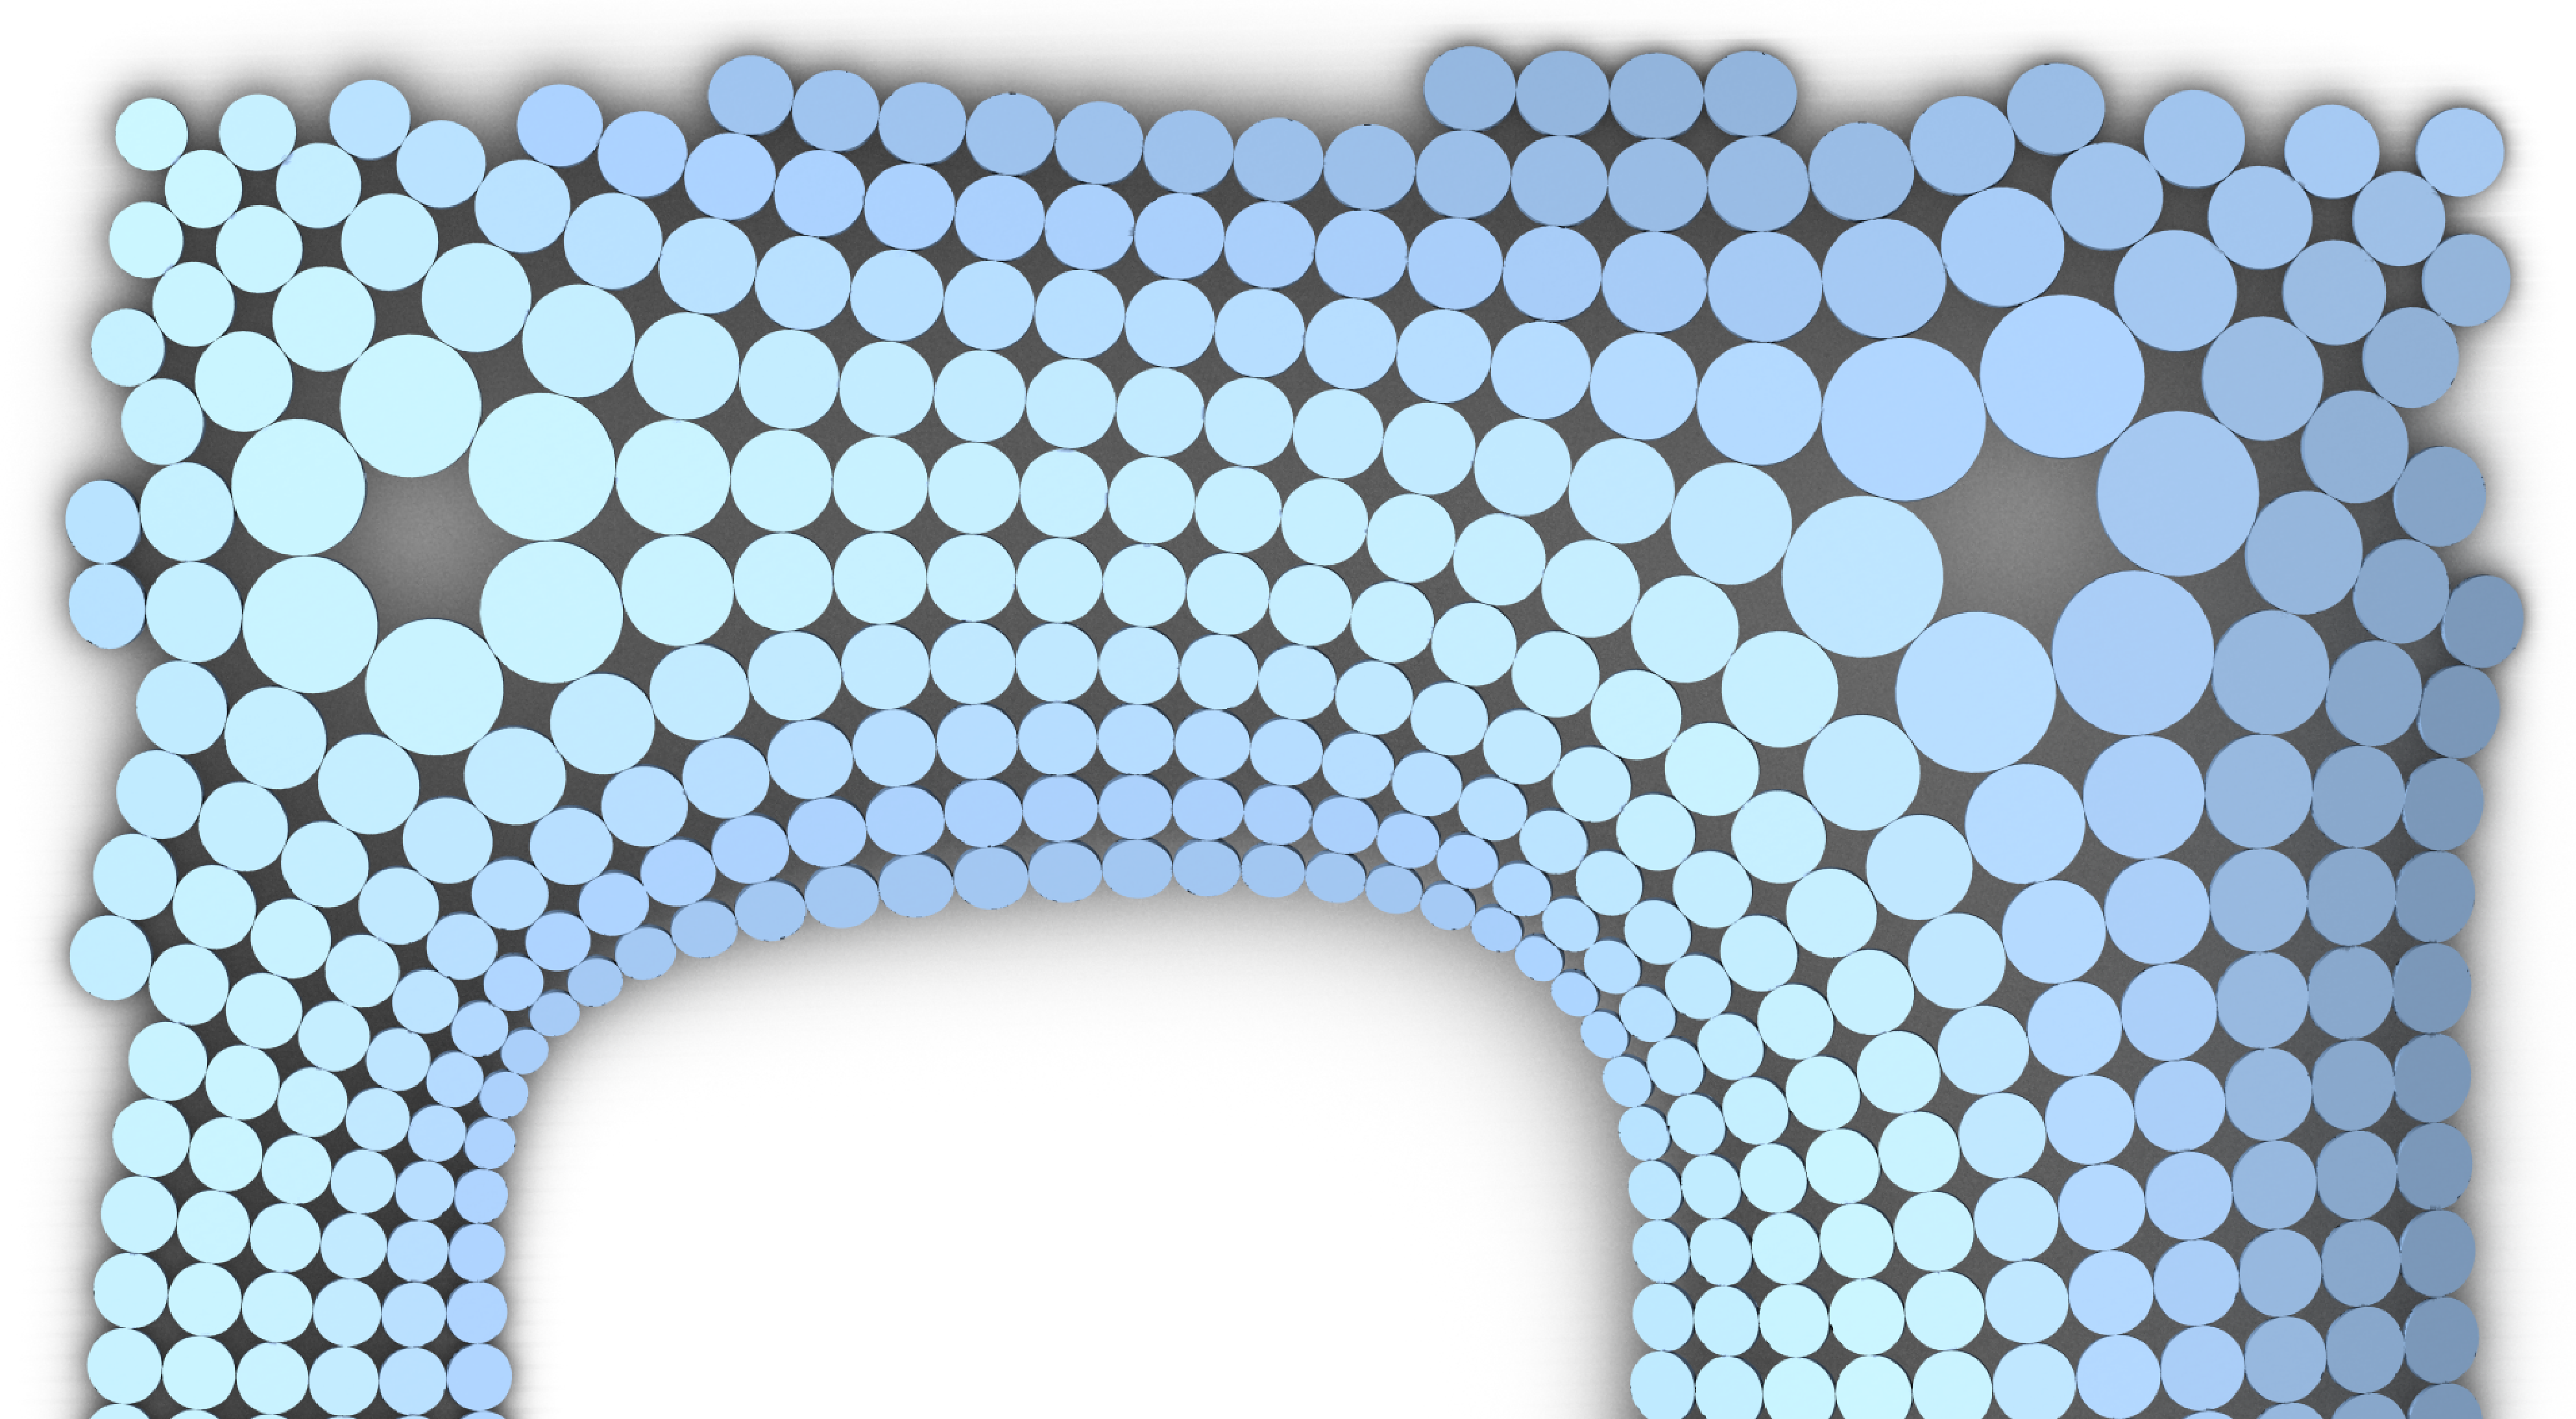
\includegraphics[height=4cm]{image/aag2012/dach_example01_circles.pdf}
%}
%\caption{
%\it Zwei Anwendungen von diskret konformen Abbildungen in der Architekturgeometrie. 
%Links: Ein Paneellayout auf einer architektonischen Fassadenoberfl\"{a}che. 
%Die Paneele sind gr\"{o}{\ss}enquantisierte regul\"{a}re Sechsecke, siehe Kapitel~2.
%Rechts: Kreismuster auf einer Dachoberfl\"{a}che.
%In Kapitel~3 berechnen wir diskrete s-isotherme Parametrisierungen f\"{u}r Fl\"{a}chen, die nahe an Isothermfl\"{a}chen sind.
%Die Ergebnisnetze haben ebene Facetten, die Kanten folgen den Hauptkr\"{u}mmungsrichtungen der Fl\"{a}che. 
%}
%\label{fig:intro_applications} 
%\end{figure}

Der zweite Teil enth\"{a}lt Anwendungen von konformen Abbildungen in der Architekturgeometrie.
In Kapitel~2 werden regul\"{a}re Muster auf architektonischen Fassaden berechnet.
Daf\"{u}r verwenden wir periodische diskret konforme Abbildungen.
Wir untersuchen, wie Randbedingungen das lokale Verhalten der Abbildungen beeinflussen.
%Am Ende verwenden wir diese Abbildungen, um die Geometrie von regul\"{a}ren Paneelen, zum Beispiel Sechsecken, zu bestimmen. 
%Wir beschreiben, wie diese Netze weiter optimiert werden um Paneele effizient produzieren zu k\"{o}nnen, siehe auch Abbildung~\ref{fig:intro_applications} links.

In Kapitel~3 nutzen wir die Tatsache aus, dass Isothermfl\"{a}chen nach Kr\"{u}mmungslinien parametrisierbar sind.
Wir berechnen s-isotherme Netze auf architektonischen Fl\"{a}chen, das sind Netze, deren ebene Facetten "sich an den Kanten ber\"{u}hrende" Kreise besitzen.
%Dieses Problem ist als Randwertproblem von diskret konformen Abbildungen formuliert.

Kapitel~4 gibt eine Einf\"{u}hrung in das Konzept der architektonischen Gitterschalen.
Geometrisch sind das Netze mit gleich langen Kanten.
Ausgehend von diskret konformen Abbildungen berechnen wir diese Strukturen mittels nicht-linearer Optimierung von Vierecksnetzen.

Der dritte Teil f\"{u}hrt den Leser in das Software-Framework ein, welches f\"{u}r Berechnungen an diskreten Fl\"{a}chen und speziell konformen Abbildungen entworfen wurde, siehe hierf\"{u}r Kapitel~8 \"{u}ber {\sc ConformalLab}.
Der Teil, der sich mit nicht-linearer Optimierung von diskreten Fl\"{a}chen besch\"{a}ftigt, ist im Kapitel~9 \"{u}ber {\sc VaryLab} beschrieben.

Der Autor hat weiter die Bibliotheken {\sc HalfEdge} and {\sc HalfEdgeTools} entworfen, siehe Kapitel~7.
Diese sind als allgemeine Werkzeuge f\"ur Berechnungen an diskreten F\"{a}chen konzipiert.
%Zusammen mit der Oberfl\"{a}chenbibliothek {\sc JRWorkspace}, Kapitel~6, bilden sie ein flexibles Framework f\"{u}r den Entwurf komplexer Forschungsanwendungen im Bereich der diskreten Differentialgeometrie.

%Diese Arbeit enth\"{a}lt eine CD mit den digitalen Daten der meisten Beispiele aus Kapitel~1 und den architektonischen Anwendungen aus Teil~II.
%Zus\"{a}tzlich ist der Quellcode der, in Teil~III beschriebenen, Software in seiner aktuellen Fassung, sowie einer kompilierten, lauff\"{a}higen Version enthalten.
%Die Struktur dieser Daten ist im Anhang beschrieben.

\subfilebibliography
\end{document}

%%% Local Variables:
%%% TeX-master: "Thesis.tex"
%%% End: